\documentclass[a4paper,10pt]{report}
\usepackage[utf8x]{inputenc}
\usepackage{graphicx}
\usepackage[brazil]{babel}
\usepackage{hyperref}
\usepackage{html,makeidx}

%specific to HTML output
%\htmltitle{Fundamentos de Computação Gráfica - INF2608}
%\htmladdress{robertogerson@telemidia.puc-rio.br}
%\htmlcss{http://www.w3.org/StyleSheets/Core/Modernist}

% Title Page
\title{Fundamentos de Computação Gráfica - INF2608}
\author{Roberto Gerson de Albuquerque Azevedo}

\begin{document}
\maketitle

\begin{abstract}
Este documento apresenta a base teórica para os trabalhos desenvolvidos no
escopo da disciplina \htmladdnormallink{Fundamentos
de Computação Gráfica (FCG) -
INF2608}{http://www.tecgraf.puc-rio.br/~mgattass/fcg/fcg.html}, cursada
durante o Doutorado em Informática pela PUC-Rio. A disciplina de FCG é subdivida
em três partes principais: Luz e Cor, Imagem e 3D. Para cada uma dessas partes é
sugerido o desenvolvimento de um projeto. As seções a seguir detalham cada um
desses projetos.
\end{abstract}

\chapter{Luz e Cor}
\par
Sendo a Computação Gráfica (CG) a área da computação destinada ao estudo de
modelos e algoritmos para o processamento de imagens digitais, o estudo da cor é
um dos seus fundamentos. A cor é uma sensação humana que os seres humanos têm
em resposta à luz incidente em nossos olhos. Sendo assim, o estudo da cor está
diretamente relacionado com o estudo da luz.

\par

\section{Enunciado do Trabalho}
\par
Um dos padrões de cor mais difundidos é o \textit{Macbeth Color Checker}
ilustrado na figura abaixo.

\begin{figure}[!htb]
     \centering
     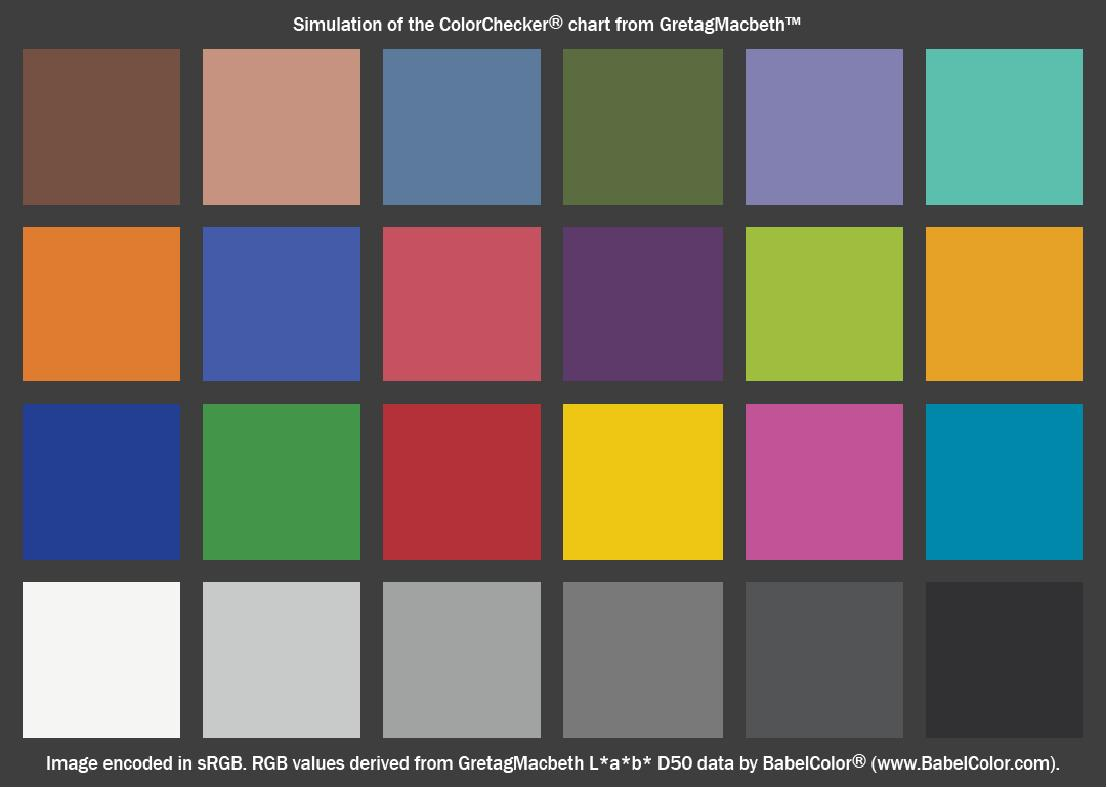
\includegraphics[scale=0.4]{img/colorChecker.jpg}
     \caption{Macbeth Color Checker. Fonte: URL}
     \label{Label de referência para a imagem}
\end{figure}

\par
Considere as amostras armazenadas por linha da esquerda para a direita de cima
para baixo.  Desta foram na última linha temos os tons de cinza e as quatro
primeiras cores são: pele escura(dark skin), pele clara(light skin), azul céu
(blue sky) e folhagem (foliage), respectivamente.  

\par
O trabalho de cor deste ano consiste em:
\newcounter{qcounter}
\begin{list}{\arabic{qcounter}:~}{\usecounter{qcounter}}
\item A partir do espectro fornecido calcular as componentes CIEXYZ,
CIExyY, CIELuv, CIELab e sRGB destas quatro primeiras amostras.
\item Somar os espectros da pele clara com o céu azul e calcular, a partir deste
novo espectro as componentes CIEXYZ, CIExyY, CIELuv, CIELab e sRGB.
\item Verificar a linearidade destes sistemas.
\end{list}

\section{Percepção da Cor}
\subsection{Observador padrão CIE}
\begin{figure}[!htb]
     \centering
     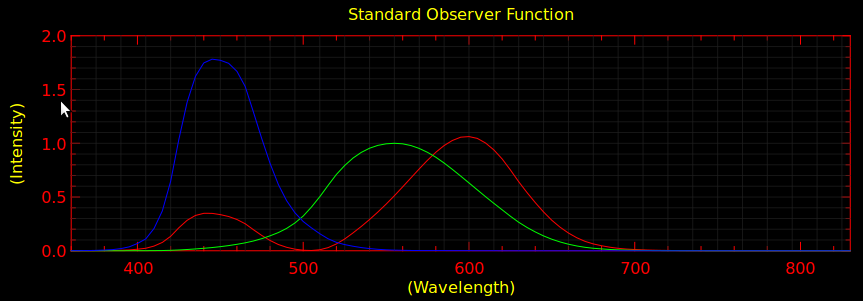
\includegraphics[scale=1.0]{img/cie_std_observer.png}
     \caption{CIE Standard Observer.}
     \label{Label de referência para a imagem}
\end{figure}

\subsection{Adaptação do sistema humano}
\par
Adaptação da visão (luz/escuro)

\par
Influência do ambiente (tamanho, cor de background etc.). Transformar a
cor de um display para que tenha a mesma aparência impressa. Outro exemplo:
dado a cor em um background, calcular a cor que "aparenta ser a mesma" e

\par
Modelos da aparência de cor. Um modelo de aparência de cor deve considerar
todas as cores em uma imagem, ao invés da cor dos pixels individualmente.

\par
Medida dos Estimulus Físicos -> Cálculo dos Três estímulos -> Cálculo dos
atributos perceptuais.

\section{Espaços de Cor}

\subsection{CIEXYZ}
Soon.

\subsection{CIExyZ}
Soon.

\subsection{CIELuv}
Soon.

\subsection{CIELab}
Soon.

\subsection{RGB}
Soon.

\subsection{sRGB}
Soon.

\section{Implementação}
Soon.

\section{Análise da Linearidade dos Espaços de Cor}
\par
Esta seção discute a linearidade dos Espaços de Cor apresentados acima, baseado
na implementação do trabalho. Para isso, primeiro temos que definir o que é um
espaço liner.
\par
Um espaço real R^n é dito linear quando, dados:

\begin{equation}\label{eqC1}
C1=(x1,x2, ..., xn)
\end{equation}

\begin{equation}\label{eqC2}
C2=(y1, y2, ..., yn)
\end{equation}

\par
pertencentes a esse espaço, pelo menos as duas propriedades a seguir são válidas
(existem algumas outras propriedades quando o espaço é de número complexos):

\begin{equation}
C_1+C_2 = (x1+y1, x_2+y_2, ..., x_n+y_n); e
\end{equation}
\begin{equation}
\item \alpha.C_1 = (\alpha.x_1, \alpha.x_2, ..., \alpha.x_n)
\end{equation}

\subsection{CIEXYZ}

\subsection{CIExyZ}
\par
Ao somar o espectro de duas cores, o resultado no sistema xyY é uma cor que está
na posição intermediária entre as cores iniciais. Se as cores originais
adicionadas estiverem na mesma proporção, teremos x resultante na média dos x's
originais e y resultante na média dos y's originais. Percebe-se assim,
claramente que estamos "misturando" a crominância das duas cores, já que ao
traçarmos uma segmento de reta entre as duas cores originais, esta nova cor
estará no ponto média deste segmento.

\par
É interessante observar também que ao somarmos os espectros de duas cores
iguais, temos como resultado a mesma cor, mas com uma luminância maior. Por
isso, as componentes de cromaticidade (x e y) são iguais ao valor original (já
que a média de dois valores iguais é ele mesmo) e o Y resultante é um valor
maior do que o Y original.

\par
Voltando ao sistema xyY, como o exemplo mostra, isso não é verdade. E, isso não
é verdade pelo fato de que x e y são sempre valores entre 0.0 e 1.0. As fórmulas
de x e y:

\begin{equation}
x=\frac{X}{X+Y+Z}
\end{equation}

\begin{equation}
y=\frac{Y}{X+Y+Z}
\end{equation}

\begin{equation}
x+y+z=1
\end{equation}

por normalizarem os valores de XYZ, já dão uma pista de que nunca poderemos ter
uma soma maior que 1.0 em uma das componentes. Por exemplo, se somarmos 0.8 +
0.8, nunca podemos ter 1.6 como resultado, invalidando a propriedade I.

\subsection{CIELuv}
Visto que o espaço de cor CIELuv é uma transformação linear do espaço xyY, é
fácil perceber que a mesma linearidade é mantida. Assim como no espaço xyY a
adição de cores resulta em uma nova cor que está na semi-reta definida pelas
duas cores iniciais.

\subsection{CIELab}
Soon.

\subsection{RGB}
Soon.

\subsection{sRGB}
Soon.

\section{Arquivos}
Soon.

\section{Instalação a partir do código-fonte}
This repository is for Roberto Azevedo's programs developed in the scope of the
Foundations of Computer Graphics discipline. This discipline was coursed during
the Roberto Doctoral course in Pontificial Catholic University of Rio de Janeiro
(PUC-Rio). Marcelo Gattass (http://www.tecgraf.puc-rio.br/~mgattass) was the
teacher.

Computer Graphics, PUC-Rio, Color, Image, 3D

\chapter{Imagem}
Soon.

\chapter{3D}
Soon.

\end{document}
